\chapter{Технологическая часть}
В этом разделе будет проведен выбор средств реализации ПО, будут приведены листинги кода и демонстрация работы программы.

\section{Средства реализации программного обеспечения}
\subsection{Выбор языка программирования}
В качестве языка программирования для реализации платформы был выбран Python 3.9, так как имеется опыт разработки проектов на этом языке. 
Также данный ЯП поддерживает парадигму ООП, соответственно, даёт возможность реализовать структуру приложения, приведённую в конструкторской части.

\subsection{Выбор СУБД}
В качестве СУБД был выбран PostgreSQL.

Postgres \cite{postgresql} -- это свободно распространяемая объектно-реляционная система управления базами данных, наиболее развитая из открытых СУБД в мире и являющаяся реальной альтернативой коммерческим базам данных \cite{postgresql-fact}.
Данная СУБД предназначена для обработки ряда рабочих нагрузок, от отдельных компьютеров до хранилищ данных или веб-сервисов с множеством одновременных пользователей. 

Выбор обусловлен тем, что имеется опыт разработки проектов с данной СУБД, а также тем, что Python и PostgreSQL являются совместимыми технологиями.

\subsection{Выбор ПО для графического интерфейса}
В качестве ПО для реализации UI был выбран среда QT по следующим причинам:
\begin{enumerate}
	\item Qt предоставляет широкую поддержку для взаимодействия с Python-приложениями.
	\item Qt является программной средой для реализации Desktop-приложений. Пользователь может воспользоваться ПО QtDesigner для разработки UI.
	\item Структура приложений QT позволяет внедрить их в ООП-архитектуру.
	\item У автора есть опыт разработки проектов с использованием QT.
\end{enumerate} 

\section{Листинги кода}

\subsection{СУБД}
На листинге 3.1 представлен код создания таблиц в базе данных:

\FloatBarrier
\begin{lstinputlisting}[language=SQL, caption=Создание таблиц в БД, 
	basicstyle=\footnotesize\ttfamily, frame=single,breaklines=true]{src/db/sql/create.sql}
\end{lstinputlisting}
\FloatBarrier

На листинге 3.2 представлен код создания ограничений на таблицы:
\FloatBarrier
\begin{lstinputlisting}[language=SQL, caption=Создание ограничений на таблицы, 
	basicstyle=\footnotesize\ttfamily, frame=single,breaklines=true]{src/db/sql/constraints.sql}
\end{lstinputlisting}
\FloatBarrier

На листинге 3.3 представлен код получения таблицы матчей в текущей линии:
\FloatBarrier
\begin{lstinputlisting}[language=SQL, caption=Получение таблицы матчей в текущей линии, linerange = {78-101},
	basicstyle=\footnotesize\ttfamily, frame=single, breaklines=true]{src/db/sql/functions.sql}
\end{lstinputlisting}
\FloatBarrier


На листинге 3.4 представлен код расчёта итога события:
\FloatBarrier
\begin{lstinputlisting}[language=SQL, caption=Расчёт итога события, linerange = {127-151},
	basicstyle=\footnotesize\ttfamily, frame=single,breaklines=true]{src/db/sql/functions.sql}
\end{lstinputlisting}
\FloatBarrier

На листинге 3.5 представлен код триггера на обновления таблицы Games, связанным с изменением состояния матча:
\FloatBarrier
\begin{lstinputlisting}[language=SQL, caption=Триггер на обновление таблицы Games, linerange = {23-50},
	basicstyle=\footnotesize\ttfamily, frame=single,breaklines=true]{src/db/sql/triggers.sql}
\end{lstinputlisting}
\FloatBarrier

На листинге 3.6 представлен код процедуры обновления баланса пользователей:
\FloatBarrier
\begin{lstinputlisting}[language=SQL, caption=Обновление балансов пользователй, linerange = {112-134},
	basicstyle=\footnotesize\ttfamily, frame=single,breaklines=true]{src/db/sql/procedures.sql}
\end{lstinputlisting}
\FloatBarrier

На листинге 3.7 представлен код выдачи прав по ролям:
\FloatBarrier
\begin{lstinputlisting}[language=SQL, caption=Выдача прав ролям, 
	basicstyle=\footnotesize\ttfamily, frame=single,breaklines=true]{src/db/sql/roles.sql}
\end{lstinputlisting}
\FloatBarrier

\subsection{Приложение}
Все действия, которые приложение может выполнить, обернуты в SQL-функции, которые затем вызываются классами, ответственными за взаимодействие с базой данных.

На листинге 3.8 представлен код выполнения SQL-запроса в Python:
\FloatBarrier
\begin{lstinputlisting}[language=Python, caption=Выполнение SQL-запроса, linerange = {11-28},
	basicstyle=\footnotesize\ttfamily, frame=single,breaklines=true]{src/db/baseRepo.py}
\end{lstinputlisting}
\FloatBarrier

На листинге 3.9 представлен код пополнения баланса пользователя:
\FloatBarrier
\begin{lstinputlisting}[language=Python, caption=Пополнение баланса пользователя, linerange = {44-47},
	basicstyle=\footnotesize\ttfamily, frame=single,breaklines=true]{src/db/playerRepo.py}
\end{lstinputlisting}
\FloatBarrier

\section{Демонстрация работы программы}
В этом разделе будут показана демонстрация работы программы в различных ситуациях.

\subsection{Вход в систему}
Стартовый экран приложения представлен на рисунке \ref{fig::start}. 
Пользователь может войти в систему, введя логин и пароль в специальном поле.
Также отсюда можно перейти к регистрации

\FloatBarrier
\begin{figure}[hp]	
	\begin{center}
		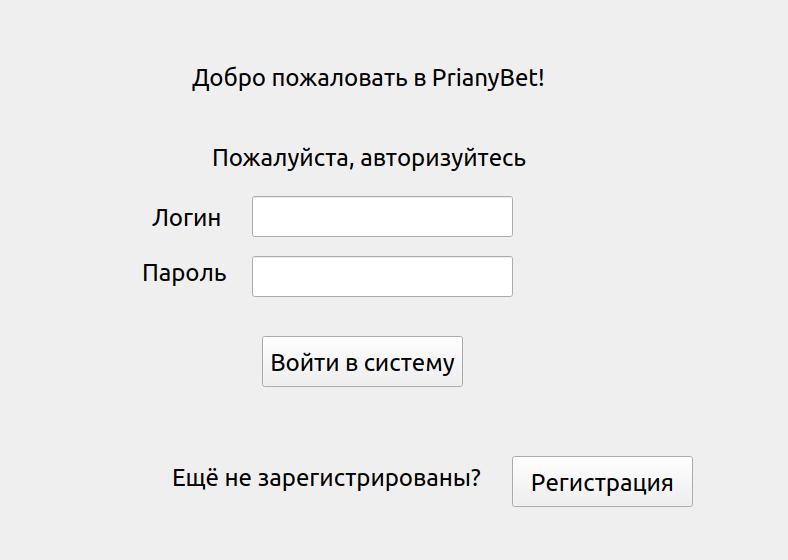
\includegraphics[width=\linewidth]{inc/start.png}
	\end{center}
	\caption{Стартовый экран приложения}
	\label{fig::start}
\end{figure}
\FloatBarrier

\subsection{Регистрация}
Экран регистрации представлен на рисунке \ref{fig::reg}. 
Пользователь вводит все данные, которые после ввода проверяются программой.
В случае успеха пользователь регистрируется в системе, либо же система выведет сообщение об ошибке.

\FloatBarrier
\begin{figure}[hp]	
	\begin{center}
		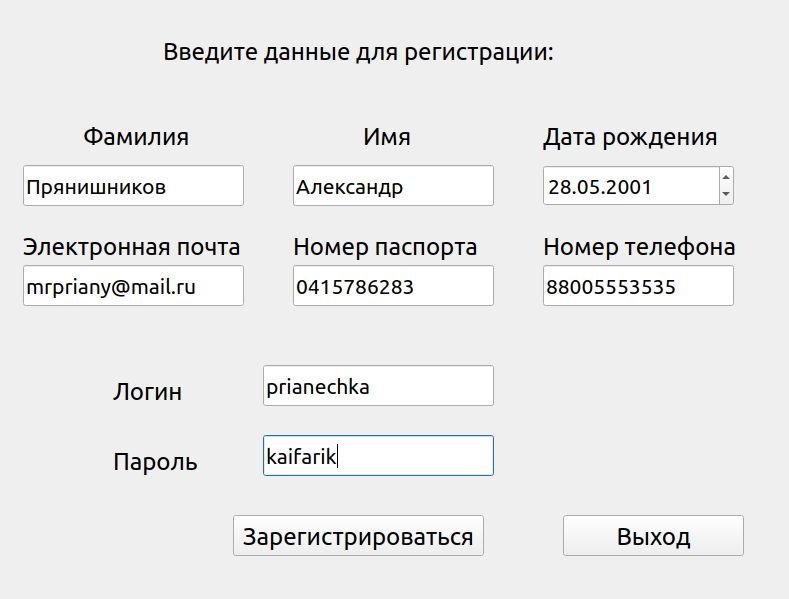
\includegraphics[width=\linewidth]{inc/registrate.png}
	\end{center}
	\caption{Экран регистрации}
	\label{fig::reg}
\end{figure}
\FloatBarrier

\subsection{Стартовое меню игрока}
Стартовый экран игрока представлен на рисунке \ref{fig::user}. 
Игрок может посмотреть сверху свои данные: баланс, логин, а также статус аккаунта.
С этого экрана можно перейти к просмотру истории ставок, пополнению баланса или непосредственно к выполнению ставок.

\FloatBarrier
\begin{figure}[hp]	
	\begin{center}
		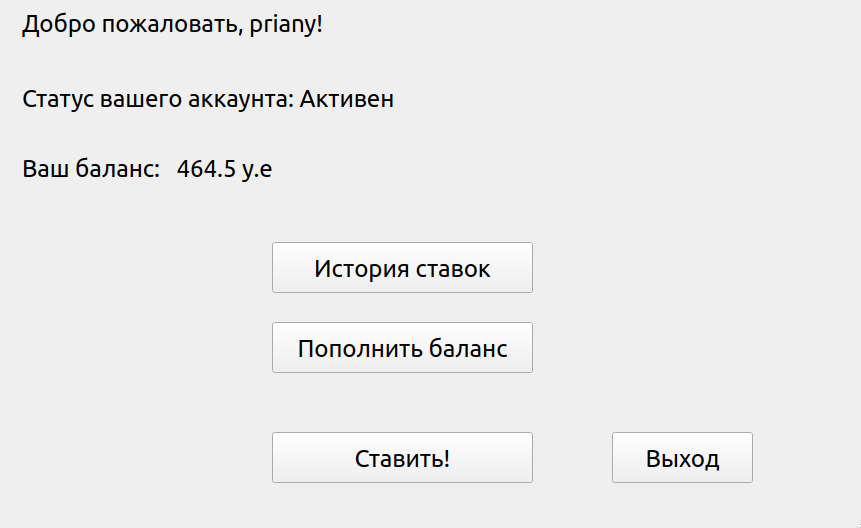
\includegraphics[width=\linewidth]{inc/user.png}
	\end{center}
	\caption{Стартовый экран игрока}
	\label{fig::user}
\end{figure}
\FloatBarrier

\subsection{Пополнение баланса}
Экран пополнения баланса представлен на рисунке \ref{fig::balance}. 
Игрок выбирает сумму пополнения, после чего при нажатии кнопки пополнения баланс успешно пополняется.

\FloatBarrier
\begin{figure}[h]	
	\begin{center}
		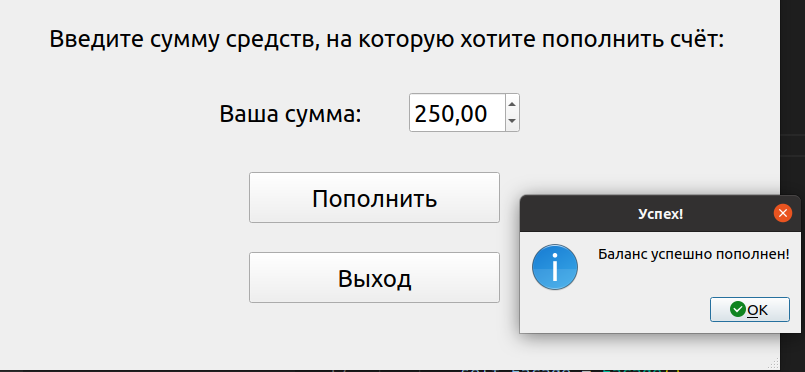
\includegraphics[height = 6cm, width=\linewidth]{inc/balance.png}
	\end{center}
	\caption{Экран пополнения баланса}
	\label{fig::balance}
\end{figure}
\FloatBarrier

\subsection{Выполнение ставок}
Экран выполнения ставок представлен на рисунке \ref{fig::bet}.

Игрок может увидеть в таблице все события, которые присутствуют в линии в данный момент.
Для выбора события, на которое нужно сделать ставку, пользователь должен выделить строку с нужным событием.
Слева внизу игрок может выбрать событие для ставки, а также сумму, на которую он хочет заключить пари.

После нажатия кнопки выполнения ставки программа оценит валидность введённых данных, и, в случае успеха, выдаст информационное сообщение.

\FloatBarrier
\begin{figure}[h]	
	\begin{center}
		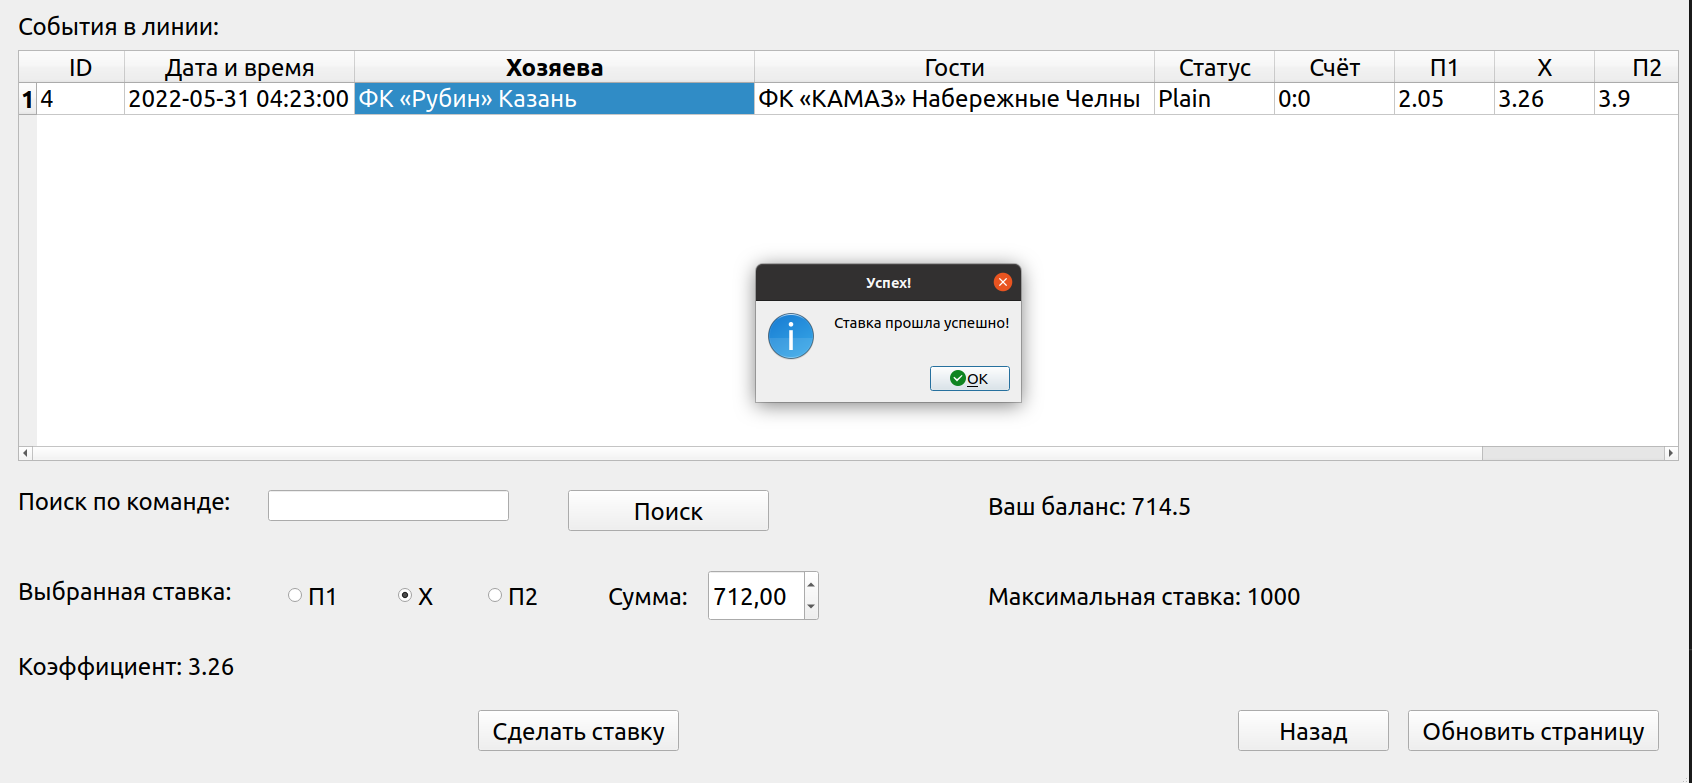
\includegraphics[height = 7cm, width=\linewidth]{inc/bet.png}
	\end{center}
	\caption{Экран выполнения ставок}
	\label{fig::bet}
\end{figure}
\FloatBarrier

\subsection{Просмотр истории ставок}
Экран просмотра истории ставок представлен на рисунке \ref{fig::history}.

Игрок может увидеть в таблице все события, которые присутствуют в линии в данный момент.
Для выбора события, на которое нужно сделать ставку, пользователь должен выделить строку с нужным событием.
Слева внизу игрок может выбрать событие для ставки, а также сумму ставки.

После нажатия кнопки выполнения ставки программа оценит валидность введённых данных, и, в случае успеха, выдаст информационное сообщение.

\FloatBarrier
\begin{figure}[h]	
	\begin{center}
		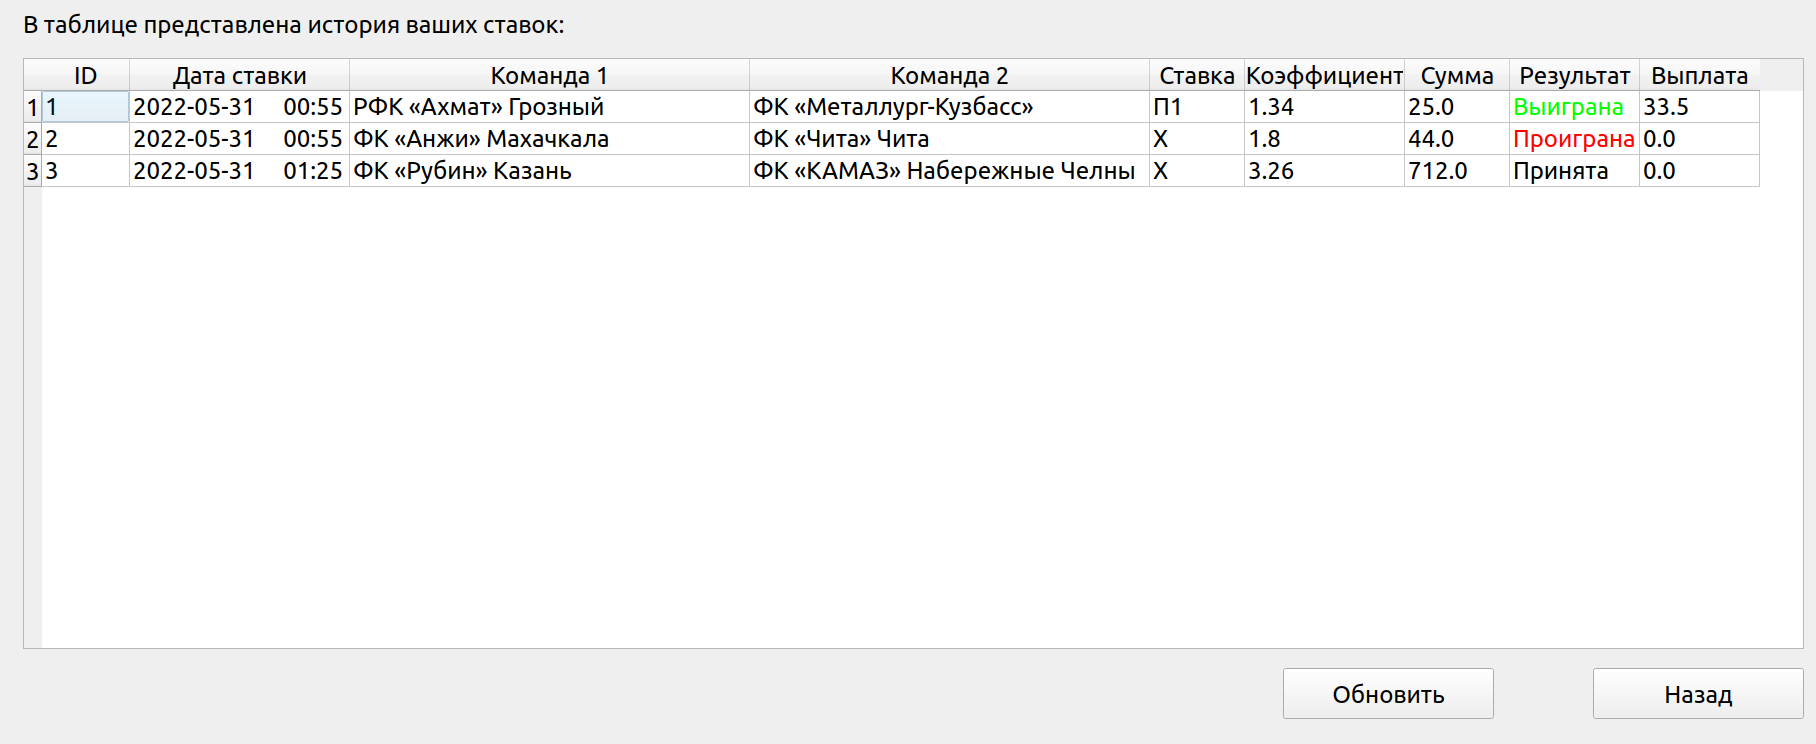
\includegraphics[width=\linewidth]{inc/history.png}
	\end{center}
	\caption{Экран просмотра истории ставок}
	\label{fig::history}
\end{figure}
\FloatBarrier

\subsection{Добавление матчей в линию аналитиком}
Экран добавления матчей в линию представлен на рисунке \ref{fig::add}.

Экран доступен только в случае входа аналитика в приложение из стартового окна.
В таблице представлен список клубов, доступных для добавления в событие.
Можно воспользоваться кнопкой поиска для нахождения клубов.
Выбор команды осуществляется нажатием на название мышкой.

Также внизу аналитик должен выбрать вероятности наступления событий. 
Сумма вероятностей должна быть равна 100\%.

\FloatBarrier
\begin{figure}[h]	
	\begin{center}
		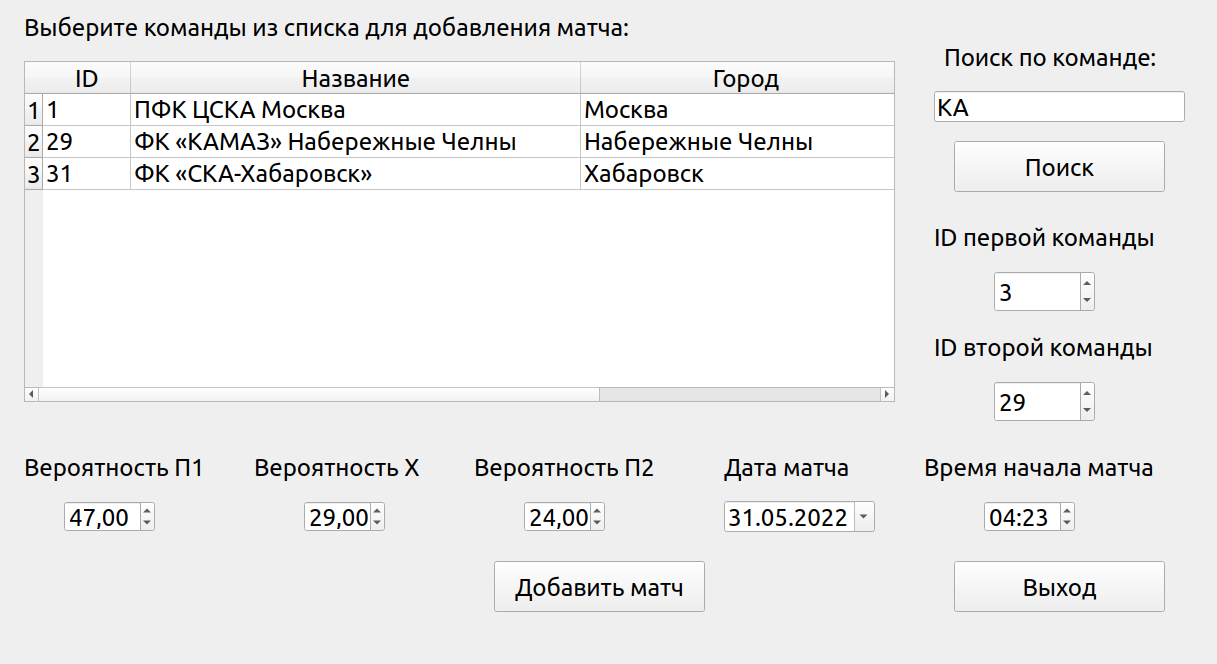
\includegraphics[width=\linewidth]{inc/addMatch.png}
	\end{center}
	\caption{Экран добавления матчей в линию}
	\label{fig::add}
\end{figure}
\FloatBarrier

\subsection{Экран изменения матчей}
Экран изменения матчей в линии представлен на рисунке \ref{fig::change}.

Экран доступен только в случае входа аналитика в приложение из стартового окна.
В таблице представлены матчи, добавленные аналитиком в предыдущем окне.
Для изменения состояния матча или изменения счёта нужно нажать на строку с событием, а затем нажать на требуемую кнопку внизу таблицы.

Также внизу аналитик может изменить вероятности наступления событий.

\FloatBarrier
\begin{figure}[h]	
	\begin{center}
		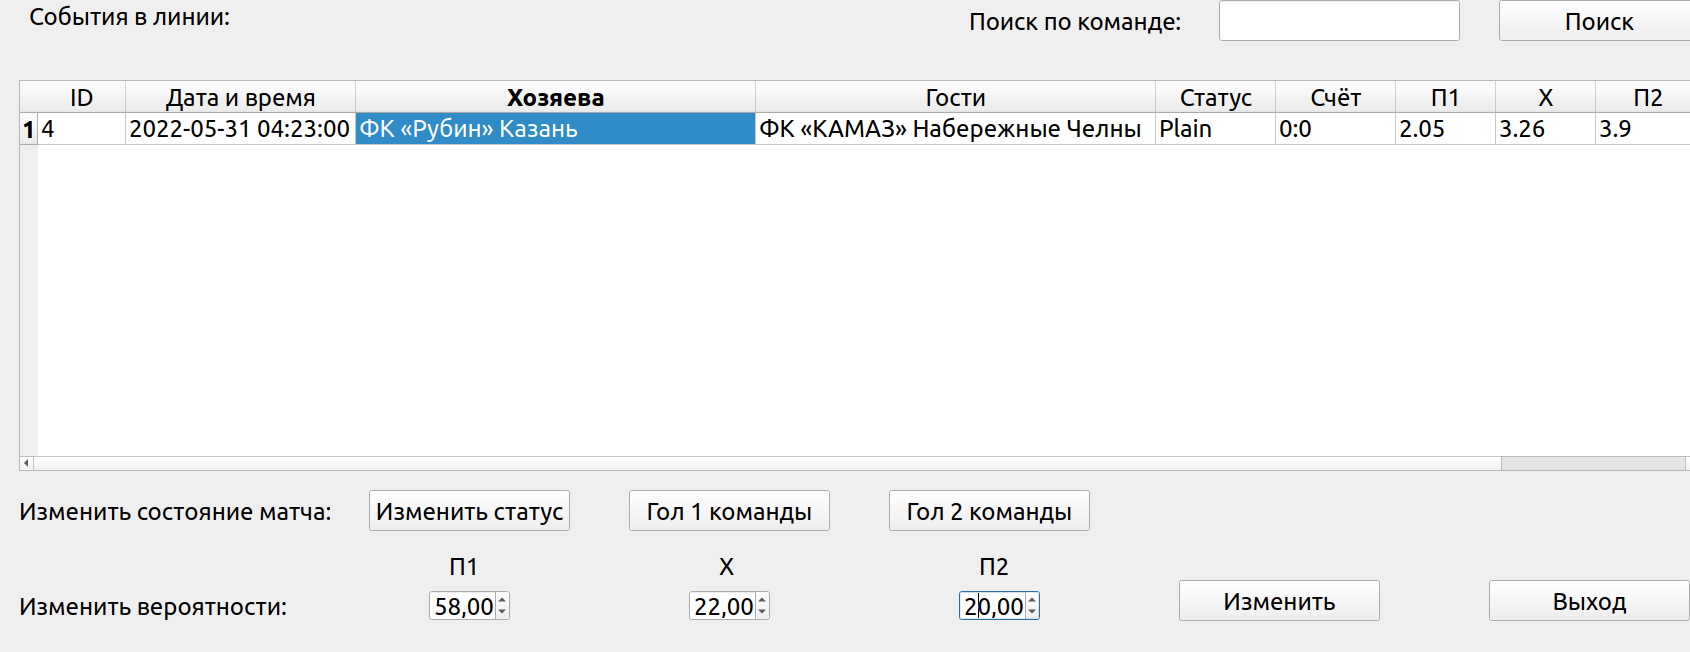
\includegraphics[height=6cm, width=\linewidth]{inc/matches.png}
	\end{center}
	\caption{Экран изменения матчей в линию}
	\label{fig::change}
\end{figure}
\FloatBarrier

\subsection{Экран верификации пользователей}
Экран верификации пользователей в линии представлен на рисунке \ref{fig::verify}.

Экран доступен только в случае входа администратора в приложение из стартового окна.
Аналитик в таблице видит список аккаунтов, которые требуют верификации.
В зависимости от введённых данных аналитик может либо верифицировать аккаунт, либо заблокировать.

\FloatBarrier
\begin{figure}[h]	
	\begin{center}
		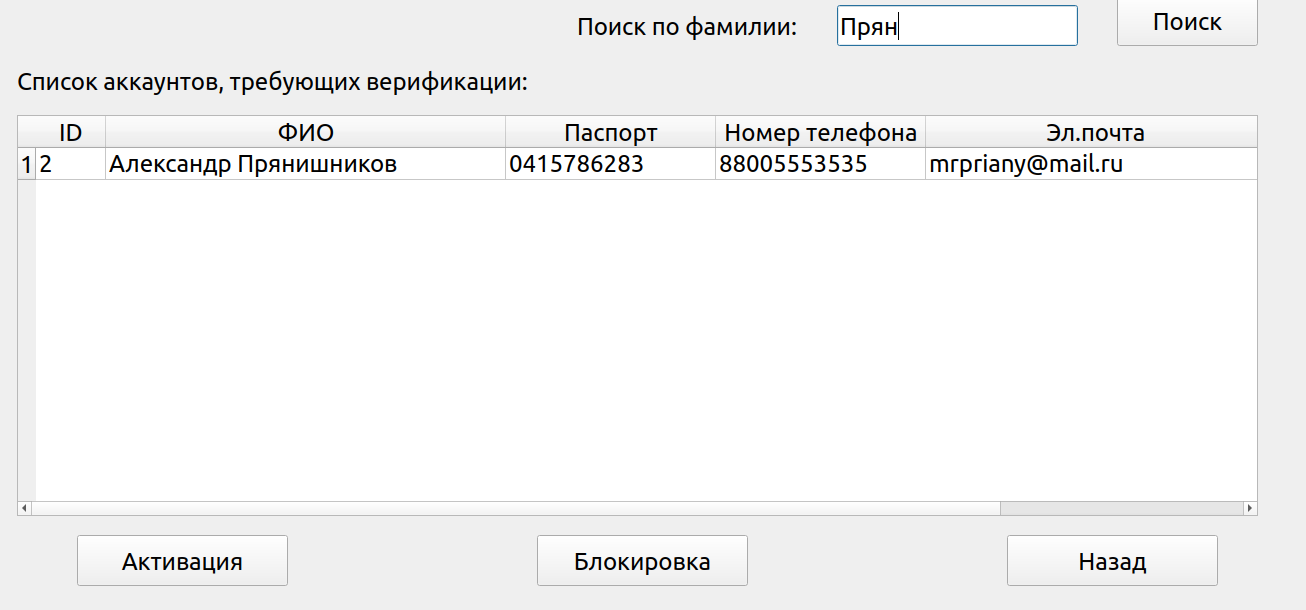
\includegraphics[width=\linewidth]{inc/verify.png}
	\end{center}
	\caption{Экран верификации пользователей}
	\label{fig::verify}
\end{figure}
\FloatBarrier